%%%%%%%%%%%%%%%%%%%%%%%%%%%%%%%%%%%%%%%%%
% a0poster Portrait Poster
% LaTeX Template
% Version 1.0 (22/06/13)
%
% The a0poster class was created by:
% Gerlinde Kettl and Matthias Weiser (tex@kettl.de)
% 
% This template has been downloaded from:
% http://www.LaTeXTemplates.com
%
% License:
% CC BY-NC-SA 3.0 (http://creativecommons.org/licenses/by-nc-sa/3.0/)
%
%%%%%%%%%%%%%%%%%%%%%%%%%%%%%%%%%%%%%%%%%

%----------------------------------------------------------------------------------------
%	PACKAGES AND OTHER DOCUMENT CONFIGURATIONS
%----------------------------------------------------------------------------------------

\documentclass[a0,portrait]{a0poster}

% increase some sizes
\renewcommand{\footnotesize}{\fontsize{20.74}{25}\selectfont}
\renewcommand{\small}{\fontsize{24.88}{30}\selectfont}
\renewcommand{\normalsize}{\fontsize{29.86}{37}\selectfont}

\usepackage{algpseudocode}
\usepackage{algorithm}
\usepackage{multicol} % This is so we can have multiple columns of text side-by-side
\columnsep=100pt % This is the amount of white space between the columns in the poster
\columnseprule=1pt % This is the thickness of the black line between the columns in the poster

\usepackage[svgnames]{xcolor} % Specify colors by their 'svgnames', for a full list of all colors available see here: http://www.latextemplates.com/svgnames-colors

\usepackage{tikz}
\usepackage{pgfplots}
% options for pgfplots
\pgfplotsset{compat=1.8,compat/show suggested version=false}
\usetikzlibrary{calc,trees,arrows,patterns,plotmarks,shapes,snakes,er,3d,automata,backgrounds,topaths,decorations.pathmorphing,decorations.markings}
%\pgfplotsset{compat=newest}
\pgfplotsset{
   /pgfplots/bar  cycle  list/.style={/pgfplots/cycle  list={%
        {black,fill=black!30!white,mark=none},%
        {black,fill=red!30!white,mark=none},%
        {black,fill=green!30!white,mark=none},%
        {black,fill=yellow!30!white,mark=none},%
        {black,fill=brown!30!white,mark=none},%
     }
   },
}
% begin of externalization
\usetikzlibrary{external}
\tikzexternalize[prefix=out/]
\tikzexternalize
% don't externalize todonotes
%\makeatletter
%\renewcommand{\todo}[2][]{\tikzexternaldisable\@todo[#1]{#2}\tikzexternalenable}
%\makeatother
% end of externalization
\usepgfplotslibrary{groupplots}
\pgfplotsset{
every axis label/.append style={font=\normalsize},
tick label style={font=\small},
}
\usepackage{times} % Use the times font
%\usepackage{palatino} % Uncomment to use the Palatino font

\usepackage{graphicx} % Required for including images
%\graphicspath{{figures/}} % Location of the graphics files
\usepackage{booktabs} % Top and bottom rules for table
\usepackage[font=normalsize,labelfont=bf]{caption} % Required for specifying captions to tables and figures
\usepackage{amsfonts, amsmath, amsthm, amssymb} % For math fonts, symbols and environments
\usepackage{wrapfig} % Allows wrapping text around tables and figures
\usepackage{subcaption}

\definecolor{mygreen}{rgb}{0,0.6,0}
\definecolor{mygray}{rgb}{0.5,0.5,0.5}
\definecolor{mymauve}{rgb}{0.58,0,0.82}
\usepackage{listings}
\lstset{ %
  backgroundcolor=\color{white},   % choose the background color; you must add \usepackage{color} or \usepackage{xcolor}
  basicstyle=\ttfamily, % the size of the fonts that are used for the code
  breakatwhitespace=false,         % sets if automatic breaks should only happen at whitespace
  breaklines=true,                 % sets automatic line breaking
  captionpos=b,                    % sets the caption-position to bottom
  commentstyle=\color{mygreen},    % comment style
  deletekeywords={...},            % if you want to delete keywords from the given language
  escapeinside={\%*}{*)},          % if you want to add LaTeX within your code
  extendedchars=true,              % lets you use non-ASCII characters; for 8-bits encodings only, does not work with UTF-8
  frame=leftline,                  % adds a frame around the code
  keepspaces=true,                 % keeps spaces in text, useful for keeping indentation of code (possibly needs columns=flexible)
  keywordstyle=\color{blue},       % keyword style
  morekeywords={*,...},            % if you want to add more keywords to the set
  numbers=left,                    % where to put the line-numbers; possible values are (none, left, right)
  numbersep=10pt,                   % how far the line-numbers are from the code
  numberstyle=\small\color{mygray}, % the style that is used for the line-numbers
  rulecolor=\color{black},         % if not set, the frame-color may be changed on line-breaks within not-black text (e.g. comments (green here))
  showspaces=false,                % show spaces everywhere adding particular underscores; it overrides 'showstringspaces'
  showstringspaces=false,          % underline spaces within strings only
  showtabs=false,                  % show tabs within strings adding particular underscores
  stepnumber=1,                    % the step between two line-numbers. If it's 1, each line will be numbered
  stringstyle=\color{black},     % string literal style
  tabsize=1,                       % sets default tabsize to 2 spaces
  title=\lstname                   % show the filename of files included with \lstinputlisting; also try caption instead of title
}

% some useful shortcuts
\newcommand{\ie}{\textit{i.e., }}
\newcommand{\eg}{\textit{e.g., }}
\newcommand{\etal}{et al.\ }
\newcommand{\CC}{C\nolinebreak\hspace{-.05em}\raisebox{.5ex}{\tiny\bf +}\nolinebreak\hspace{-.10em}\raisebox{.5ex}{\tiny\bf +}}

% units for results
\newcommand{\uj}{\,$\mu$J}
\newcommand{\mw}{\,mW}
\newcommand{\uw}{\,$\mu$W}
\newcommand{\ns}{\,ns}
\newcommand{\us}{\,$\mu$s}
\newcommand{\ms}{\,ms}
\newcommand{\KB}{\,KB}
\newcommand{\MB}{\,MB}
\newcommand{\GB}{\,GB}
\newcommand{\MHz}{\,MHz}
\newcommand{\GHz}{\,GHz}

% \newcommand{\SYSTEM}{Bard}
% \newcommand{\system}{bard}
% new latex commands:
%   Remove long section
\newcommand{\PUNT}[1]{}

%   Referencing various pieces of the document:
\newcommand{\figref}[1]{Figure~\ref{fig:#1}}
\newcommand{\figsref}[2]{Figures~\ref{fig:#1} and~\ref{fig:#2}}
\newcommand{\figrref}[2]{Figures~\ref{fig:#1}--\ref{fig:#2}}
\newcommand{\secref}[1]{Section~\ref{sec:#1}}
\newcommand{\secsref}[2]{Sections~\ref{sec:#1} and~\ref{sec:#2}}
\newcommand{\eqnref}[1]{Eqn.~\ref{eqn:#1}}
\newcommand{\eqnsref}[2]{Eqns.~\ref{eqn:#1} and~\ref{eqn:#2}}
\newcommand{\eqnrref}[2]{Eqns.~\ref{eqn:#1}--\ref{eqn:#2}}
\newcommand{\insref}[1]{Instruction~\ref{ins:#1}}
\newcommand{\tblref}[1]{Table~\ref{tbl:#1}}
\newcommand{\appref}[1]{Appendix~\ref{app:#1}}
\newcommand{\algoref}[1]{Algorithm~\ref{algo:#1}}

\newcommand{\argmin}{\arg\!\min}
\newcommand{\argmax}{\arg\!\max}
\newcommand{\minimize}{minimize}
\newcommand{\optimize}{optimize}
\newcommand{\st}{s.t.}

\newcommand{\app}[1]{\mbox{\texttt{#1}}}
\newcommand{\interface}[1]{\textbf{#1}}
\newcommand{\function}[1]{\mbox{\texttt{#1}}}
\newcommand{\struct}[1]{\emph{#1}}
\newcommand{\variable}[1]{\emph{#1}}

\newcommand{\PAD}{\vskip 0.75cm}

\usepackage[natbib=true,backend=bibtex,firstinits=true,style=numeric-comp,sorting=nyt,defernumbers,maxnames=2,maxcitenames=2,doi=false,isbn=false,url=false]{biblatex}
\bibliography{seec}

% Use bold for vectors instead of arrows
\renewcommand{\vec}[1]{\mathbf{#1}}

\begin{document}

%----------------------------------------------------------------------------------------
%	POSTER HEADER 
%----------------------------------------------------------------------------------------

\begin{minipage}[b]{\linewidth}
\begin{center}

\includegraphics[height=5cm]{figures/uchicago_logo.png} %[width=20cm]
\hspace{42cm}

\includegraphics[height=5cm]{figures/lbnl_logo.png}\\
\vspace{0.5cm}
\noindent\makebox[\linewidth]{\rule{0.9\paperwidth}{0.4pt}}
\vspace{0.5cm}
\end{center}

\Huge \color{NavyBlue} \textbf{Energy Efficiency in HPC with Machine Learning and Control Theory} \color{Black}\\[0.5cm] % Title
% \veryHuge \color{NavyBlue} \textbf{Bard} \color{Black}\\[0.5cm] % Title
% \Huge\textit{A Unified Framework for Managing Soft Timing and Power Constraints}\\[1.5cm] % Subtitle
%\begin{center}
\huge \textbf{Connor Imes, Steven Hofmeyr, and Henry Hoffmann}\\[0.25cm] % Author(s)
\LARGE \textbf{ckimes@cs.uchicago.edu, shofmeyr@lbl.gov, hankhoffmann@cs.uchicago.edu}
% \\
% \Large \textbf{University of Chicago, Lawrence Berkeley National Laboratory*} % University/organization
%\end{center}
\end{minipage}
%

%\vspace{1cm} % A bit of extra whitespace between the header and poster content

%----------------------------------------------------------------------------------------

\begin{multicols}{2} % This is how many columns your poster will be broken into, a portrait poster is generally split into 2 columns

%----------------------------------------------------------------------------------------
%	ABSTRACT
%----------------------------------------------------------------------------------------

\color{Navy} % Navy color for the abstract

\begin{abstract}

\normalsize
Performance and power management in High Performance Computing (HPC) has historically favored a race-to-idle approach in order to complete applications as quickly as possible, often wasting a significant amount of energy.
As we move toward exascale and hardware over-provisioning, power management is becoming more critical than ever for HPC system administrators, opening the door for more balanced approaches to performance and power management.
We propose two projects to address balancing application performance and system power consumption in HPC \emph{during application runtime}, using closed loop feedback designs based on the Self-aware Computing Model to \emph{observe}, \emph{act}, and \emph{decide}.

{
\PAD
\centering
  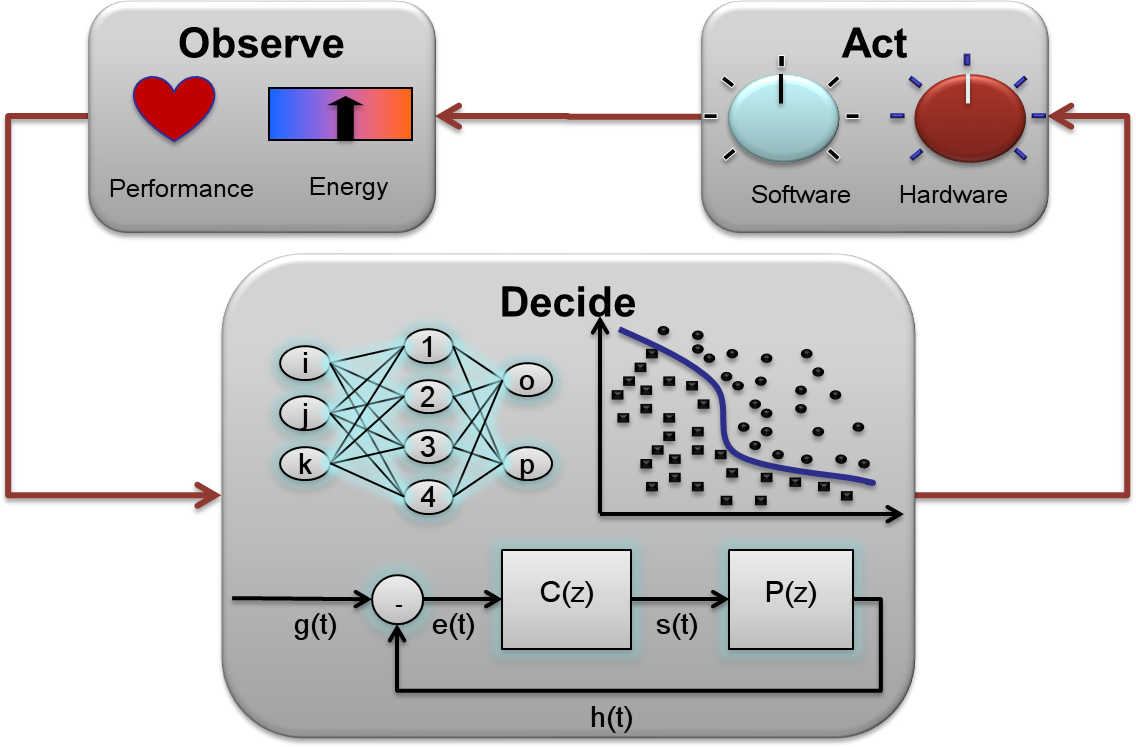
\includegraphics[width=0.8\columnwidth]{figures/seec.png}
  \captionof{figure}{The Self-aware Computing Model.}
  \label{fig:runtime-ee}
\PAD
}

\end{abstract}

%----------------------------------------------------------------------------------------
%	INTRODUCTION
%----------------------------------------------------------------------------------------

%\color{SaddleBrown} % SaddleBrown color for the introduction

%\section*{Introduction}

%----------------------------------------------------------------------------------------
%	OBJECTIVES
%----------------------------------------------------------------------------------------

\color{DarkSlateGray} % DarkSlateGray color for the rest of the content

% \vspace{-1cm}
% \section*{Motivation}


%----------------------------------------------------------------------------------------
%	MATERIALS AND METHODS
%----------------------------------------------------------------------------------------

\vspace{-1cm}
\section*{Machine Learning Classification for Energy Efficiency}

\textbf{Dynamic voltage and frequency scaling (DVFS)} is effective at saving energy by scaling back the processor during I/O or on code that is off the critical path.
DVFS is available in HPC job schedulers, though unfortunately today it is typically only configurable when a job is launched.

We propose a \interface{Machine Learning-based classifier} to predict the most energy-efficient DVFS frequencies \emph{during runtime} to maximize the work-to-cost ratio of an application running on a single node.
To train and drive our classifier, we capture low-level \emph{hardware counter metrics}, available through tools like \app{PAPI} and \app{PCM}.

{
\PAD
\centering
  \tikzset{%
  app/.style    = {draw, thin, rectangle, minimum height = 2.5em,
    minimum width = 5em, fill=black!25},
  block/.style    = {draw, thick, rectangle, minimum height = 3em,
    minimum width = 5em},
  blockres/.style    = {draw, thick, rectangle, minimum height = 3em,
    minimum width = 5em, fill=green!25},
  biblock/.style  = {draw, thick, rectangle, minimum height = 6em,
    minimum width = 6em, fill=red!25},
  sum/.style      = {draw, circle, node distance = 4cm}, % Adder
  input/.style    = {coordinate}, % Input
  output/.style   = {coordinate} % Output
}

\begin{tikzpicture}[scale=1.0,transform shape, auto, thick, node distance=1.5cm, >=triangle 45]

\draw
  % Drawing the top blocks
  % node [input, name=goalaccuracy] {} 
  % node [left of=goalaccuracy, node distance=0.35mm]{}
  % node [sum, right of=goalaccuracy] (sumaccuracy) {} % negative feedback
  node [block, align=center] (featureselection) 
    {Feature\\Selection}
  node [block, right of=featureselection, align=center, node distance=12cm] (classifier) 
    {Classifier}
  node [blockres, above of=classifier, align=center, node distance=5cm] (trainingdata) 
    {Training\\Data}
;
  % Connectng lines
% \draw[->](goalaccuracy) -- node[align=center] {Timing\\Goal}(sumaccuracy);
% \draw[->](sumaccuracy) -- node[align=center] {Timing\\Error}(featureselection);
\draw[->](featureselection) -- node[align=center] {Processed\\Data}(classifier);
\draw[->](trainingdata) -- (classifier);

% Draw software system
\draw
  node [biblock, right of=classifier, node distance=12cm, align=center, yshift=-1cm] (system)
    {\\System\\\\\\}
;
\draw
  node [app, right of=classifier, node distance=12cm, align=center, yshift=-2cm] (software)
    {Application}
;

% lines from translators to software
\draw[->](classifier.east) -- node [name=ka,align=center]{System\\Settings} (classifier.east -| system.west);

% Connectng lines
\coordinate (feedbackup) at ([yshift=-2cm]featureselection.south);
\draw (system.west |- feedbackup) -| node [near end,align=center] {PCM\\Sample} (feedbackup);
\draw[->](feedbackup) -- node[pos=0.99] {} (featureselection);

\end{tikzpicture}
  \captionof{figure}{\interface{Machine Learning Classifier} closed loop feedback control design.}
  \label{fig:runtime-ee}
\PAD
}

At regular time intervals, the classifier predicts the most energy-efficient frequency to use based on measured application behavior, then applies the setting to the system.
% At regular time intervals, \eg every second, the classifier makes a new prediction.
As applications move through \emph{phases}, the controller adapts to the changing application and system behavior.
For example, we test a parallel video encoder:

{
\PAD
\centering
  \begin{tikzpicture}
\begin{centering}

\definecolor{s1}{RGB}{228, 26, 28}
\definecolor{s2}{RGB}{55, 126, 184}
\definecolor{s3}{RGB}{77, 175, 74}
\definecolor{s4}{RGB}{152, 78, 163}
\definecolor{s5}{RGB}{255, 127, 0}

\begin{groupplot}[
    group style={
        group name=plots,
        group size=1 by 2,
        xlabels at=edge bottom,
        xticklabels at=edge bottom,
        vertical sep=10pt
    },
height=8cm,
width=0.8\columnwidth,
xmajorgrids,
ymajorgrids,
grid style={dashed},
xmin=0,
xmax=60,
yticklabel pos=left,
enlargelimits=false,
tick align = outside,
tick style={white},
xticklabel shift={-5pt},
yticklabel shift={-5pt},
ylabel shift={-2pt},
ylabel style={align=center},
unbounded coords=jump,
]

\nextgroupplot[ylabel={DVFS \\ Frequency \\ (Normalized)}, % Performance
xtick={0,5,10,15,20,25,30,35,40,45,50,55,60},
ytick={0.0,0.2,0.4,0.6,0.8,1.0},
yticklabels={0.0,0.2,0.4,0.6,0.8,1.0},
% yticklabel style={font=\footnotesize},
ymin=0.5,
ymax=1.1,
% legend entries={{\footnotesize $\mathsf{Server}$}},
% legend style={draw=none,at={(0.5,1.4)},anchor=north,legend columns=4,line width=5pt},
]
\addplot[ultra thick, solid, color=s2] table[x index=0,y index=1,col sep=tab] {img/x264-phases-ee.txt};
\addplot[thick, solid, black] coordinates {(0, 1) (60, 1)};
% \addplot[thick, dashed, black] coordinates {(1500,0) (1500, 2)};
% \addplot[thick, dashed, black] coordinates {(3000,0) (3000, 2)};


\nextgroupplot[ylabel={Energy \\ Efficiency \\ (Normalized)}, % Power
ytick={0.0,0.2,0.4,0.6,0.8,1.0,1.2,1.4},
yticklabels={0.0,0.2,0.4,0.6,0.8,1.0,1.2,1.4},
% yticklabel style={font=\footnotesize},
ymin=0,
ymax=1.4,
xlabel={$time$ [seconds]},
xlabel near ticks,
xtick={0,5,10,15,20,25,30,35,40,45,50,55,60},
xticklabels={0,,10,,20,,30,,40,,50,,60},
% xticklabel style={font=\footnotesize},
]
\addplot[ultra thick, solid, color=s1] table[x index=0,y index=2,col sep=tab] {img/x264-phases-ee.txt};
\addplot[thick, solid, black] coordinates {(0, 1) (60, 1)}; % race
% \addplot[thick, solid, black] coordinates {(0, 0.773) (60, 0.773)}; % worst-case
% \addplot[thick, dashed, black] coordinates {(1500,0) (1500, 250)};
% \addplot[thick, dashed, black] coordinates {(3000,0) (3000, 250)};

\end{groupplot}
\end{centering}

\end{tikzpicture}
    
  \captionof{figure}{Energy-efficient video encoding (Support Vector Machine classifier).}
  \label{fig:classifier-phases-x264-ee}
\PAD
}

% \vfill\null
% \columnbreak

%------------------------------------------------

%\subsection*{Mathematical Section}



%----------------------------------------------------------------------------------------
% RESULTS 
%----------------------------------------------------------------------------------------

\vspace{-1cm}
\section*{MIMO Controller for Power Balancing}

In recent years, hardware has been taking more direct control of processor voltage and frequency, making fine-tuned software-management of DVFS obsolete.
Fine-grained \interface{power capping} is now the preferred mechanism for managing performance and power tradeoffs, evidenced by the introduction of power capping implementations like \interface{Intel Running Average Power Limit (RAPL)} and the move from Speed Step to Speed Shift.

Nodes in HPC clusters suffer \emph{non-uniformity} in performance and power consumption due to both manufacturing process variation and imbalance in application workloads.
We propose a generalized \interface{Multiple Input, Multiple Output (MIMO) Proportional Integral Derivative (PID) controller} to shift power allocations between nodes to eliminate tail idle times in job iterations, thus maximizing application throughput while respecting a global power cap.
Unlike heuristic approaches to power management, \textbf{control theory} provides \emph{formal guarantees} of \emph{convergence} as well as \emph{robustness} to application, system, and measurement noise.
These guarantees hold even for applications with different \emph{phases}.

{
\PAD
\centering
  \tikzset{%
  app/.style    = {draw, thin, rectangle, minimum height = 2.5em,
    minimum width = 5em, fill=black!25},
  block/.style    = {draw, thick, rectangle, minimum height = 3em,
    minimum width = 5em},
  blockres/.style    = {draw, thick, rectangle, minimum height = 3em,
    minimum width = 5em, fill=green!25},
  biblock/.style  = {draw, line width=0.15cm, rectangle, minimum height = 6em,
    minimum width = 6em, fill=red!25},
  sum/.style      = {draw, circle, node distance = 4cm}, % Adder
  input/.style    = {coordinate}, % Input
  output/.style   = {coordinate} % Output
}

\tikzstyle{vecArrow} = [thick, decoration={markings,mark=at position
   1 with {\arrow[semithick]{open triangle 60}}},
   double distance=1.4pt, shorten >= 5.5pt,
   preaction = {decorate},
   postaction = {draw,line width=1.4pt, white,shorten >= 4.5pt}]
\tikzstyle{vecLine} = [thick, double distance=1.4pt, shorten >= 5.5pt]
\tikzstyle{innerWhite} = [semithick, white,line width=1.4pt, shorten >= 4.5pt]

\begin{tikzpicture}[scale=1.0,transform shape, auto, thick, node distance=1.5cm, >=triangle 45]

\draw
  % Drawing the top blocks
  node [input, name=goalaccuracy] {} 
  node [left of=goalaccuracy, node distance=0.35mm]{}
  node [sum, right of=goalaccuracy] (sumaccuracy) {} % negative feedback
  node [block, right of=sumaccuracy, align=center, node distance=10cm] (controlaccuracy) 
    {~Controller~}
  % node [block, right of=controlaccuracy, align=center, node distance=3.0cm] (translateaccuracy) 
  %   {Mapper}
  % node [blockres, above of=controlaccuracy, align=center, node distance=5cm] (resourcefile) 
  %   {Initial\\Power Caps}
;
  % Connectng lines
\draw[vecArrow](goalaccuracy) -- node[align=center] {Reference\\Idle Times\\($\vec{0}$)}(sumaccuracy);
\draw[vecArrow](sumaccuracy) -- node[align=center] {Relative\\Timing\\Error}(controlaccuracy);
% \draw[->](controlaccuracy) -- node[align=center] {Generic\\Control\\Signal}(translateaccuracy);
% \draw[vecArrow](resourcefile) -- (controlaccuracy);

% Draw software system
\draw
  node [biblock, right of=controlaccuracy, node distance=12cm, align=center, yshift=-1cm] (system)
    {\\System\\\\\\}
;
\draw
  node [app, right of=controlaccuracy, node distance=12cm, align=center, yshift=-2cm] (software)
    {Distributed\\Application}
;

% lines from translators to software
\draw[vecArrow](controlaccuracy.east) -- node [name=ka,align=center]{Power\\Caps} (controlaccuracy.east -| system.west);

% Connectng lines
\coordinate (feedbackup) at ([yshift=-2cm]sumaccuracy.south);
\draw[vecLine](software.west |- feedbackup) -| node [near end,align=center] {\\Measured\\Idle Times} (feedbackup);
\draw[vecArrow](feedbackup) -- node[pos=0.99] {$-$} (sumaccuracy);

\draw[innerWhite](software.west |- feedbackup) -| node [near end,align=center] {} (feedbackup);
% \draw[innerWhite](feedbackup) -- node[pos=0.99] {} (sumaccuracy);

\end{tikzpicture}
  \captionof{figure}{\interface{MIMO PID controller} closed loop feedback control design.}
  \label{fig:runtime-nlpb}
\PAD
}

Given a cluster with $n$ nodes and global power cap $\Gamma$, the PID controller computes a new power signal vector $\vec{u}$ of size $n$ in each iteration $t$:
\begin{eqnarray}
\vec{u}(t) = \vec{u}(t-1) + K_I \cdot \vec{e}(t)
\end{eqnarray}
$K_I$ is the ratio of control change and $\vec{e}(t)$ are the node idle times, divided by their mean and normalized around $0$.
This formulation ensures that the entire global power cap is re-allocated in each iteration.
Formally:
\begin{eqnarray}
\sum_{i=1}^{n} e_i(t) = 0 \implies \sum_{i=1}^{n} u_i(t) = \sum_{i=1}^{n} u_i(t-1) = \Gamma
\end{eqnarray}
$K_I$ is currently a fixed scalar value decided at initialization time, but we are exploring ways to predict it dynamically at runtime, \eg using a Kalman filter.

We simulate meeting a global power cap of 180 Watts on an artificially imbalanced quad-socket system ($\Gamma=180$, $n=4$) using a MPI+OpenMP application, with each MPI process bound to a socket.
We begin with evenly distributed power caps, \ie $u_i(0) = \frac{\Gamma}{n}$ for each socket $i$.
We then run 10 time steps:

% \begin{minipage}{\columnwidth}
% \PAD
% \centering
% \begin{tabular}{|c|c|c|c|c|c|}
% \hline
% \textbf{} & \textbf{Iteration 0} & \textbf{Iteration 1} & \textbf{Iteration 2} & \textbf{Iteration 3} & \textbf{Iteration 4} \\
% \hline
% \textbf{Node 0} & 100 & 105 & 105 & 106 & 103 \\
% \textbf{Node 1} & 100 & 97  & 96  & 97  & ... \\
% \textbf{Node 2} & 100 & 96  & 98  & 97  & ... \\
% \textbf{Node 4} & 100 & 102 & 101 & 100 & ... \\
% \hline
% \textbf{Sum}    & 400 W & 400 W & 400 W & 400 W & 400 W \\
% \hline
% \end{tabular}
% \captionof{table}{Example of balancing 1 400 Watt power cap between 4 nodes.}
% \label{tbl:nlpb-example}
% \PAD
% \end{minipage}

{
% NLPB_K=2.5 ./nlpb-simulator -n 4 -g 180 -p 40 -P 70 -c /local/nlpb-scripts/boggle/omp-only-balanced-3ghz-rapl.results -i boggle_imbalance.txt -N 10 -l nlpb.log
% boggle_imbalance:.txt
% 0.8
% 0.92
% 1.10
% 1.18
\PAD
\centering
  \begin{tikzpicture}
\begin{centering}

\definecolor{s1}{RGB}{228, 26, 28}
\definecolor{s2}{RGB}{55, 126, 184}
\definecolor{s3}{RGB}{77, 175, 74}
\definecolor{s4}{RGB}{152, 78, 163}
\definecolor{s5}{RGB}{255, 127, 0}

\begin{groupplot}[
    group style={
        group name=plots,
        group size=1 by 2,
        xlabels at=edge bottom,
        xticklabels at=edge bottom,
        vertical sep=10pt
    },
height=8cm,
width=0.8\columnwidth,
xmajorgrids,
ymajorgrids,
grid style={dashed},
xmin=0,
xmax=10,
yticklabel pos=left,
enlargelimits=false,
tick align = outside,
tick style={white},
xticklabel shift={-5pt},
yticklabel shift={-5pt},
ylabel shift={-2pt},
ylabel style={align=center},
unbounded coords=jump,
legend cell align=left, 
legend style={ column sep=1ex },
]


\nextgroupplot[ylabel={Idle Time (S)}, % Performance
% xlabel={$time$ [iteration]},
% xlabel near ticks,
xtick={0,1,2,3,4,5,6,7,8,9,10},
ytick={0,2,4,6,8,10,12,14},
yticklabels={0,2,4,6,8,10,12,~~~14},
% yticklabel style={font=\footnotesize},
ymin=0,
ymax=14,
legend entries={{$\mathsf{Process~0}$},{$\mathsf{Process~1}$},{$\mathsf{Process~2}$},{$\mathsf{Process~3}$}},
legend style={draw=none,at={(0.5,1.25)},anchor=north,legend columns=4,line width=5pt},
]
\addplot[ultra thick, solid, color=s1] table[x index=0,y index=10,col sep=space] {img/nlpb.log};
\addplot[ultra thick, solid, color=s2] table[x index=0,y index=13,col sep=space] {img/nlpb.log};
\addplot[ultra thick, solid, color=s3] table[x index=0,y index=16,col sep=space] {img/nlpb.log};
\addplot[ultra thick, solid, color=s4] table[x index=0,y index=19,col sep=space] {img/nlpb.log};
\addplot[thick, solid, black] coordinates {(0, 45) (10, 45)};
% \addplot[ultra thick, dashed, black] coordinates {(1500,0) (1500, 2)};
% \addplot[ultra thick, dashed, black] coordinates {(3000,0) (3000, 2)};

\nextgroupplot[ylabel={Power Cap (W)}, % Performance
xlabel={$time$ [iteration]},
xlabel near ticks,
xtick={0,1,2,3,4,5,6,7,8,9,10},
ytick={44,44.25,44.5,44.75,45,45.25,45.5,45.75,46,46.25,46.5},
yticklabels={44.0,,44.5,,45.0,,45.5,,46.0,,},
% yticklabel style={font=\footnotesize},
ymin=44,
ymax=46.5,
% legend entries={{$\mathsf{Process~0}$},{$\mathsf{Process~1}$},{$\mathsf{Process~2}$},{$\mathsf{Process~3}$}},
% legend style={draw=none,at={(0.5,1.2)},anchor=north,legend columns=4,line width=5pt},
]
\addplot[ultra thick, solid, color=s1] table[x index=0,y index=12,col sep=space] {img/nlpb.log};
\addplot[ultra thick, solid, color=s2] table[x index=0,y index=15,col sep=space] {img/nlpb.log};
\addplot[ultra thick, solid, color=s3] table[x index=0,y index=18,col sep=space] {img/nlpb.log};
\addplot[ultra thick, solid, color=s4] table[x index=0,y index=21,col sep=space] {img/nlpb.log};
\addplot[thick, solid, black] coordinates {(0, 45) (10, 45)};
% \addplot[ultra thick, dashed, black] coordinates {(1500,0) (1500, 2)};
% \addplot[ultra thick, dashed, black] coordinates {(3000,0) (3000, 2)};


\end{groupplot}
\end{centering}

\end{tikzpicture}
    
  \captionof{figure}{Simulation of changing node power caps between iterations.}
  \label{fig:nlpb-sim}
\PAD
}

The controller quickly re-balances power caps so that nodes finish their jobs with near-zero tail idle times.

Some outstanding issues remain to be addressed:
\begin{itemize}
\item Handling node-level minimum and maximum power bounds.
\item Estimating $K_I$ at runtime.
\item Properly and accurately measuring tail idle times in MPI processes.
\item Gaining access to a cluster that supports runtime power cap adjustments.
\end{itemize}

%----------------------------------------------------------------------------------------
%	CONCLUSIONS
%----------------------------------------------------------------------------------------
\color{SaddleBrown} % SaddleBrown color for the conclusions to make them stand out

% \section*{Conclusions}



\color{DarkSlateGray} % Set the color back to DarkSlateGray for the rest of the content

%----------------------------------------------------------------------------------------
%	FORTHCOMING RESEARCH
%----------------------------------------------------------------------------------------

%\section*{Forthcoming Research}



 %----------------------------------------------------------------------------------------
%	REFERENCES
%----------------------------------------------------------------------------------------

% \printbibliography
%\nocite{*} % Print all references regardless of whether they were cited in the poster or not
%\bibliographystyle{plain} % Plain referencing style
%\bibliography{seec}

%----------------------------------------------------------------------------------------
%	ACKNOWLEDGEMENTS
%----------------------------------------------------------------------------------------

\PUNT{
\section*{Acknowledgements}

\footnotesize
The effort on this project is funded by the U.S. Government under the DARPA BRASS program, by the Dept. of Energy under DOE DE-AC02-06CH11357, by the NSF under CCF 1439156, and by a DOE Early Career Award.
}

%----------------------------------------------------------------------------------------

\end{multicols}

% \begin{minipage}[b]{\linewidth}
\begin{center}
\vspace{0.5cm}
\Large \texttt{https://people.cs.uchicago.edu/{\raise.17ex\hbox{$\scriptstyle\mathtt{\sim}$}}ckimes/}
% \Large \texttt{http://poet.cs.uchicago.edu/}~~~~~~$\vert$~~~~~~\texttt{http://github.com/energymon/}~~~~~~$\vert$~~~~~~\texttt{http://github.com/powercap/}
\end{center}
% \end{minipage}

\end{document}